\documentclass[tikz,border=7pt]{standalone}
\begin{document}
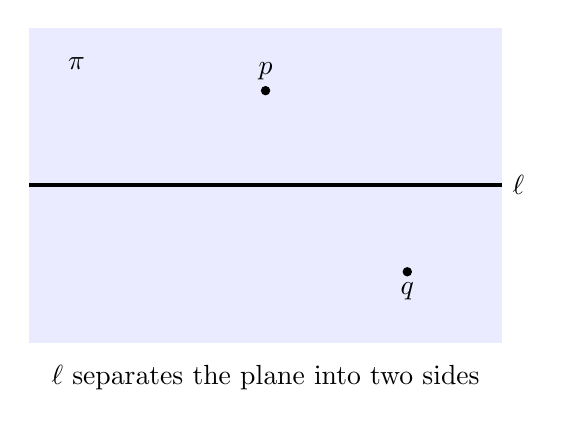
\begin{tikzpicture}[line width=.8pt]
\fill[blue!8] (-3,-2) rectangle (3,2); \draw[very thick] (-3,0)--(3,0) node[right] {$\ell$};
\fill (0,1.2) circle (1.7pt) node[above] {$p$}; \fill (1.8,-1.1) circle (1.7pt) node[below] {$q$};
\node at (-2.4,1.55) {$\pi$}; \node at (0,-2.45) {$\ell$ separates the plane into two sides};
\end{tikzpicture}
\end{document}
